\newpage
\chapter{Landasan Kepustakaan}

Landasan kepustakaan berisi uraian dan pembahasan tentang teori, konsep, model, metode, atau sistem dari pustaka ilmiah, yang berkaitan dengan tema, masalah, atau pertanyaan penelitian. Dalam landasan kepustakaan terdapat landasan teori dari berbagai sumber pustaka yang terkait dengan teori dan metode yang digunakan dalam penelitian. Jika dibutuhkan sesuai dengan karakteristik penelitiannya dan syarat kecukupan khusus keminatan tertentu, bisa juga terdapat kajian pustaka yang menjelaskan secara umum penelitian-penelitian terdahulu yang berhubungan dengan topik skripsi dan menunjukkan persamaan dan perbedaan skripsi tersebut terhadap penelitian terdahulu yang dituliskan. 

\section{Subbab Dua Satu}

Isi landasan kepustakaan bukanlah sekedar salinan dari sumber pustaka, tetapi merupakan ringkasan, sintesis, atau kombinasi dari keduanya, terhadap informasi dari sumber pustaka. Ringkasan adalah uraian singkat dari hal-hal yang relevan dari sumber pustaka (Brown, 2005), sedangkan sintesis adalah reorganisasi atau penyusunan ulang berbagai informasi yang relevan tersebut sehingga secara keseluruhan membentuk kerangka teoritik dari penelitian (Richmod, 2005).

\subsection{Subbab Dua Satu Satu}

Dalam membuat ringkasan, informasi teoritik yang dipilih dari sumber pustaka haruslah yang benar-benar relevan dengan masalah penelitian. Oleh karena itu, peneliti harus kritis dalam menyeleksi informasi. Kemudian, untuk menjaga agar informasi yang dipilih memang berasal dari studi atau kajian ilmiah, disarankan menggunakan sumber-sumber pustaka ilmiah, seperti jurnal, prosiding konferensi atau seminar, tesis, disertasi, skripsi, atau buku teks, dan dihindari sumber-sumber yang tidak jelas penulisnya atau kapasitas penulisnya. Jika informasi yang diambil dimaksudkan untuk pembahasan teori, konsep, atau metode terkini, maka sebaiknya sumber yang digunakan adalah yang semutakhir mungkin.

Menurut Berndtsson et al. (2008), dalam melakukan sintesis, informasi teoritik sebaiknya dijelaskan mulai dari informasi yang lebih umum dan secara bertahap menuju ke yang lebih khusus. Penulis juga seharusnya menjelaskan aspek-aspek mana dari informasi teoritik tersebut yang langsung berhubungan atau menjadi dasar dari masalah penelitian, serta bagaimana aspek tersebut berhubungan dengan masalah penelitian (Rumbaugh et al., 2005; Brodjonegoro, 2009a; Sommerville, 2011).

\subsection{Subbab Dua Satu Dua}

Ketika harus mengacu informasi dari sumber pustaka, penulis wajib memberikan apresiasi kepada penulis pustaka tersebut dengan cara menuliskan identitas pustaka tersebut beserta penulisnya dalam Daftar Pustaka dan mereferensi informasi tersebut dari badan tulisan dengan cara yang tepat.

Dalam berbagai laporan atau artikel ilmiah, landasan kepustakaan atau tinjauan kepustakaan dapat menjadi sebuah bab sendiri atau isinya menjadi bagian dari satu atau lebih bab yang lain. Selain itu, judul bab/subbab yang dipakai juga bervariasi, diantaranya adalah yang bersifat tematik. Oleh karena itu, jika diperlukan, judul bab Landasan Kepustakaan dalam skripsi juga dapat digantikan dengan judul lain yang tematik dan deskriptif terhadap isi dari bab tersebut.

\section{Subbab Dua Dua}

Penulisan persamaan, tabel, gambar, dan symbol-simbol memiliki aturan khusus seperti yang dijelaskan dalam subbab-subbab berikut.

\subsection{Subbab Dua Dua Satu tentang Persamaan}

Setiap   persamaan   yang   digunakan   harus   diberi   nomor   berurutan  berdasar bab dan urutan munculnya persamaan. Huruf pertama suatu persamaan dimulai setelah 10 ketikan spasi dari batas kiri. Nomor persamaan ditulis di kanan persamaan dan ditempatkan pada batas kanan halaman dalam tanda kurung. Bilangan pertama menunjukkkan bab letak persamaan tersebut dan bilangan kedua yang dipisahkan tanda hubung merupakan nomor urutan persamaan dalam bab tersebut. Contoh persamaan ke-10 dalam bab kedua adalah:
           							(2.10)
Ketika persamaan ini diacu dari dalam teks maka dapat dituliskan sebagai Persamaan 2.10. 

\subsection{Subbab Dua Dua Dua tentang Tabel}

Tabel berguna untuk menyajikan informasi yang detil dalam jumlah banyak. Setiap tabel memiliki nomor urut dan judul yang diletakkan di atas tabel. Nomor urut tabel terdiri atas nomor bab dan nomor urut kemunculan tabel itu dalam bab yang bersangkutan. Kedua nomor ini dipisahkan dengan titik. Penulisan nomornya serupa dengan penulisan nomor persamaan. Antara nomor tabel dan judul tabel dipisahkan oleh satu ketikan spasi. Judul tabel ditulis secara ringkas dan jelas, diawali dengan huruf kapital, diikuti dengan huruf kecil, tanpa diakhiri tanda titik, dan ditulis tebal (bold). Penulisan kata "Tabel" dalam naskah yang disertai dengan nomor tabel harus diawali dengan huruf kapital seperti pada contoh berikut: 

\begin{table}
  \caption{Pembentukan bilangan random untuk Indeks Masa Tubuh (IMT)}
  \centering
  \renewcommand{\arraystretch}{1.2}
  \begin{tabular}[ht]{clc}
    \hline
    No & Keanggotaan IMT & Rentang Nilai \\
    \hline
    1 & Sangat Kurus & 0.0 - 19.0 \\
    2 & Kurus & 15.0 - 20.0 \\
    3 & Normal & 17.0 - 27.0 \\
    4 & Gemuk & 23.0 - 29.0 \\
    5 & Obesitas & 25.0 - 50.0 \\
    \hline
  \end{tabular}
\end{table}

Judul tabel harus berada dalam satu halaman dengan tabelnya. Selain itu, sebuah tabel sebaiknya diusahakan untuk termuat dalam satu halaman, tidak terpenggal ke dalam lebih dari satu halaman. Untuk menghindari pemenggalan tabel, ukuran huruf dan spasi kata-kata dalam tabel dapat diperkecil tetapi harus tetap terbaca. 

Jika terpaksa dipenggal, tabel yang sama pada halaman berikutnya harus tetap diberi identitas di atasnya. Identitas ini terdiri dari kata "Tabel", no tabel, judul tabel (opsional) dan kata "(lanjutan)", misalnya:

Tabel 2.1 (lanjutan)  

atau

Tabel 2.2 Judul tabel (lanjutan)

Judul setiap kolom juga tetap harus dituliskan pada penggalan tabel di halaman berikutnya. Fitur yang relevan dalam program pengolah kata dapat digunakan untuk menjaga konsistensi ini. 

Contoh tabel yang terpaksa harus terpenggal dapat dilihat pada Tabel 2.2.

% \begin{table}
  % \renewcommand{\arraystretch}{1.2}
  \begin{longtable}{cl}
    
    \caption{Contoh tabel 2} \\
    % \renewcommand{\arraystretch}{1.2}
    % \begin{longtable}[h]{cl}
      \hline
      No & Nama Universitas di Indonesia \\
      \hline
      \endfirsthead
      \caption{Contoh tabel 2 (lanjutan)} \\
      \hline
      No & Nama Universitas di Indonesia \\
      \hline
      \endhead
      \hline
      \endfoot
      1 & Universitas 1 \\
      2 & Universitas 2 \\
      3 & Universitas 3 \\
      4 & Universitas 4 \\
      5 & Universitas 5 \\
      6 & Universitas 6 \\
      7 & Universitas 7 \\
      8 & Universitas 8 \\
      9 & Universitas 9 \\
      10 & Universitas 10 \\
      11 & Universitas 11 \\
      12 & Universitas 12 \\
      13 & Universitas 13 \\
      14 & Universitas 14 \\
      15 & Universitas 15 \\
      16 & Universitas 16 \\
      17 & Universitas 17 \\
      18 & Universitas 18 \\
      19 & Universitas 19 \\
      20 & Universitas 20 \\
      21 & Universitas 21 \\
      22 & Universitas 22 \\
      23 & Universitas 23 \\
      24 & Universitas 24 \\
      25 & Universitas 25 \\
      26 & Universitas 26 \\
      27 & Universitas 27 \\
      28 & Universitas 28 \\
      29 & Universitas 29 \\
      30 & Universitas 30 \\
      31 & Universitas 31 \\
      32 & Universitas 32 \\
      33 & Universitas 33 \\
      \hline
  \end{longtable}
% \end{table}

Jika sebuah tabel harus disajikan dalam bentuk landscape, maka bagian atas tabel harus diletakkan di sebelah kiri. Dalam hal ini nomor halaman harus tetap di tengah bawah.   

Jika sebuah tabel berasal dari sumber pustaka lainnya, maka sumber tersebut harus dituliskan sebagai referensi dalam daftar referensi dan sitasi terhadap referensi itu dituliskan di bawah tabel. Penjelasan lebih lanjut tentang sitasi gambar beserta contohnya dapat dilihat pada buku panduan. 

Sebuah tabel tidak berdiri sendiri tanpa teks yang merujuknya. Tabel dapat menggambarkan data yang disebutkan dalam teks atau sebaliknya teks dapat menjelaskan bagaimana data dalam tabel dilihat dan dianalisis. Tabel yang berada pada lampiran juga tetap harus dirujuk dari dalam bagian utama.

\subsection{Gambar}

Gambar dalam skripsi dapat meliputi diagram, grafik, peta, foto, dan sebagainya. Sebagaimana tabel, setiap gambar memiliki nomor urut dan judul. Tetapi berbeda dengan tabel, nomor urut dan judul gambar diletakkan di bawah gambar. Nomor urut gambar terdiri atas nomor bab dan nomor urut kemunculan gambar tersebut dalam bab yang bersangkutan. Kedua nomor ini dipisahkan dengan titik. Penulisan nomornya serupa dengan penulisan nomor tabel. Antara nomor gambar dan judul gambar dipisahkan oleh satu ketikan spasi. Judul gambar ditulis secara ringkas dan jelas, diawali dengan huruf kapital, diikuti dengan huruf kecil, tanpa diakhiri tanda titik, dan ditulis tebal (bold). Penulisan kata "Gambar" dalam naskah yang disertai dengan nomor gambar harus diawali dengan huruf kapital seperti pada Gambar  2.1 berikut. 

\begin{figure}[ht]
  \centering
  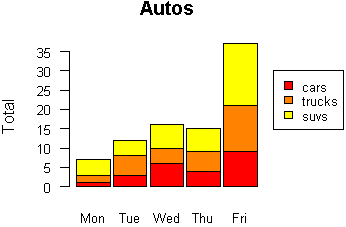
\includegraphics[width=.5\textwidth]{babs/images/bar_script4.png}
  \caption{Pengaruh nilai K terhadap akurasi}
  \label{fig:pengaruh}
\end{figure}


Judul tabel harus berada dalam satu halaman dengan tabelnya. Fitur yang relevan dalam program pengolah kata dapat digunakan untuk menjaga konsistensi ini.

Jika sebuah gambar harus disajikan dalam bentuk landscape, maka bagian atas gambar harus diletakkan di sebelah kiri. Dalam hal ini nomor halaman harus tetap berada di tengah bawah.   

Jika sebuah gambar berasal dari sumber pustaka lainnya, maka sumber tersebut harus dituliskan sebagai referensi dalam daftar referensi dan sitasi terhadap referensi itu dituliskan di bawah gambar. Penjelasan tentang sitasi gambar beserta contohnya dapat dilihat pada buku panduan skripsi. 

Gambar berwarna sebaiknya dicetak berwarna atau diatur dengan pewarnaan yang kontras. Gambar yang dikutip dari sumber lain atau hasil pemindaian (scan) hendaknya diperhatikan tingkat resolusi dan ketajamannya.  

Sebuah gambar tidak berdiri sendiri tanpa teks yang merujuknya. Gambar dapat mengilustrasikan apa yang disebutkan dalam teks atau sebaliknya teks dapat menjelaskan apa yang berada dalam gambar. Gambar yang berada pada lampiran juga tetap harus dirujuk dari teks dalam bagian utama.

\subsection{Lambang, Satuan, dan Singkatan}

Penulisan lambang atau simbol sebaiknya menggunakan fasilitas simbol atau jenis huruf Symbol yang ada pada program komputer pengolah kata untuk membedakannya dengan huruf biasa. Sebagai contoh untuk tanda perkalian tidak menggunakan huruf x tetapi "$\times$" dari symbol. Untuk rumus matematika diusahakan ditulis dalam satu baris. Bila hal ini tidak memungkinkan maka harus diatur sedemikian rupa agar mudah dimengerti.
Satuan dan singkatan yang digunakan adalah yang lazim dipakai dalam disiplin ilmu terkait, misalnya 25°C; 10 ppm; H2O; dan sebagainya. Superscript dan subscript sebaiknya digunakan ketika diperlukan. 

\subsection{Subbab Dua Dua Satu Tentang Sitasi Tabel dan Gambar}

Tabel atau gambar yang direproduksi dari sumber lain, baik itu disalin langsung secara keseluruhan, atau diadaptasi (misalnya, disesuaikan bentuk dan formatnya, atau ditambahkan keterngan legenda dengan tidak mengubah arti), harus dibuatkan referensinya dalam daftar referensi dan sitasinya di bawah tabel atau gambar tersebut.

Contoh:

Referensi dalam daftar referensi:

\begin{displayquote}
  \bibentry{anggariawan:2014} 
\end{displayquote}

\begin{table}
  \centering
  \renewcommand{\arraystretch}{1.2}
  \caption{Pembentukan bilangan random untuk Indeks Masa Tubuh (IMT). Sitasi untuk tabel yang disalin langsung.}
  \begin{tabular}{clc}
    \hline
    No & Keanggotaan IMT & Rentang Nilai \\
    \hline
    1 & Sangat Kurus & 0.0 - 19.0 \\
    2 & Kurus & 15.0 - 20.0 \\
    3 & Normal & 17.0 - 27.0 \\
    4 & Gemuk & 23.0 - 29.0 \\
    5 & Obesitas & 25.0 - 50.0 \\
    \hline
    \multicolumn{2}{l}{\footnotesize{Sumber: \cite{anggariawan:2014}}} \\
  \end{tabular}
\end{table}




\begin{table}
  \centering
  \renewcommand{\arraystretch}{1.2}
  \caption{Pembentukan bilangan random untuk Indeks Masa Tubuh (IMT). Sitasi untuk tabel yang diadaptasi.}
  \begin{tabular}{clc}
    \hline
    No & Keanggotaan IMT & Rentang Nilai \\
    \hline
    1 & Sangat Kurus & 0.0 - 19.0 \\
    2 & Kurus & 15.0 - 20.0 \\
    3 & Normal & 17.0 - 27.0 \\
    4 & Gemuk & 23.0 - 29.0 \\
    5 & Obesitas & 25.0 - 50.0 \\
    \hline
    \multicolumn{2}{l}{\footnotesize{Sumber: Diadaptasi dari \cite{anggariawan:2014}}} \\
  \end{tabular}
\end{table}

Jika tabel atau gambar adalah hasil perujukan sekunder, maka penulisan sitasi mengikuti aturan perujukan sekunder. Contohnya:
\begin{displayquote}
  Sumber: \cite{anggariawan:2014} disitasi dalam \cite{Bloggs1950}
\end{displayquote}

Penulisan istilah "Sumber" hanya digunakan jika tabel atau gambar berasal dari sumber lainnya sehingga perlu dilakukan sitasi. Jika tabel atau gambar adalah hasil karya penulis sendiri, tentu tidak diperlukan sitasi dan penulisan sumber.

\subsection{Subbab Dua Dua Dua}

Berikut ini adalah contoh penggunaan daftar beberapa pernyataan yang tersusun bernomor dan yang berindeks alfabetik:

\begin{enumerate}
  \item Aspek satu berkaitan dengan: 
  \begin{enumerate}[label=\alph*.]
    \item Aspek satu a
    \item Aspek satu b 
  \end{enumerate}
  \item Aspek dua berkaitan dengan: 
  \begin{enumerate}[label=\alph*.]
    \item Aspek dua a
    \item Aspek dua b
    \item Aspek dua c 
  \end{enumerate}
\end{enumerate}

Aspek-aspek tersebut bisa dijelaskan lebih lanjut sesuai tujuan dan kebutuhan. Penulisan di atas adalah sebuah contoh. 

\subsection{Kode Sumber}

Kode sumber (source code) dapat dituliskan dalam bagian utama atau lampiran skripsi hanya jika benar-benar dibutuhkan untuk memperjelas solusi yang diusulkan. Penulisannya dibatasi hanya pada bagian-bagian yang terpenting, misalkan metode atau algoritme utama yang digunakan. Akan tetapi lebih disarankan untuk menggantinya dengan pseudocode atau notasi lainnya. Hal ini karena penulisan kode sumber yang berlebihan hanya mempertebal skripsi tanpa memberikan nilai tambah. Selain itu, kode sumber tersebut sebenarnya termasuk properti intelektual penulis yang seharusnya dilindungi. 

Jika terpaksa harus dituliskan, kode sumber menggunakan tipe huruf Courier New berukuran 9 dan berspasi single. Kemudian, kode sumber dimasukkan ke dalam kolom ke-2 sebuah tabel yang dilengkapi dengan nomor baris di kolom ke-1. Contoh penulisan kode sumber adalah sebagai berikut: 

\noindent\textbf{\textit{Algoritme 1: Fungsi Iteratif}}
\begin{Verbatim}[numbers=left,xleftmargin=5mm,fontsize=\small]
public static void main(String[] args) {    
  int first = 10, second = 20;
  System.out.println(first + " " + second);

  // add two numbers
  int sum = first + second;
  System.out.println("The sum is: " + sum);
}
\end{Verbatim}

\noindent Without line numbering

\noindent\textbf{\textit{Algoritme 2: Fungsi Iteratif}}

\begin{Verbatim}[fontsize=\small]
public static void main(String[] args) {    
  int first = 10, second = 20;
  System.out.println(first + " " + second);

  // add two numbers
  int sum = first + second;
  System.out.println("The sum is: " + sum);
}
\end{Verbatim}